\section{Evaluation}
\label{sec:evaluation}

In the first part of this section, we analyze different kinds of ontologies and datasets
and investigate the usability of the results proposed above.
In the second part, we evaluate the implementation of Algorithm~$\mathsf{A}_{\text{prc}}$
and compare it to the reasoning system RDFox.

\subsection{Practical Usability of the Theoretical Results}

In this part, we analyze different kinds of ontologies and datasets
including benchmarks, real-world ontologies and
datasets that can be expressed in ontology languages.
Based on the analysis of these datasets,
we find that, ignoring imports, many of them
belong to $\mathcal{D}_{\textit{\text{dhl}}}$ or
$\mathcal{D}_{\textit{\text{dhl}}(\circ)}$.

\textbf{Benchmarks}. In the
Semantic Web community, many benchmarks are proposed to
facilitate the evaluation of ontology-based systems
in a standard and systematic way. We investigate several
popular benchmarks using our results. For some benchmarks, the ontologies have TBoxes with a simple
structure. These ontologies can be expressed in RDFS
and belong to $\mathcal{D}_{\textit{\text{dhl}}}$.
These benchmarks include SIB\footnote{https://www.w3.org/wiki/Social$\underline{~}$Network$\underline{~}$Intelligence$\underline{~}$BenchMark}
(\emph{Social Network Intelligence BenchMark}),
BSBM\footnote{http://wifo5-03.informatik.uni-mannheim.de/bizer/berlinsparqlbenchmark/}
(\emph{Berlin SPARQL Benchmark}) and
LODIB\footnote{http://wifo5-03.informatik.uni-mannheim.de/bizer/lodib/}
(\emph{Linked Open Data Integration Benchmark}).
The ontology used in IIMB\footnote{http://islab.di.unimi.it/iimb/}
(\emph{The ISLab Instance Matching Benchmark}) satisfies the simple-concept restriction.

In the latest version of LUBM\footnote{http://swat.cse.lehigh.edu/projects/lubm/}
(The Lehigh University Benchmark),
there are 48 classes and 32 properties.
Statements about properties, such as inverse property statements,
can be rewritten into datalog rules allowed in $\mathcal{D}_{\textit{\text{dhl}}}$.
Most of the statements about classes can be rewritten into datalog rules that
are allowed in $\mathcal{D}_{\textit{\text{dhl}}}$.
Five axioms have, however, the form $A\sqsubseteq\exists R.B$,
which requires existentially quantified variables in the rule head when rewriting
the axiom into a logic rule: $A(x)\rightarrow\exists y(R(x,y)\wedge B(y))$,
where a new anonymous constant $y$ is introduced.
This kind of rule is not considered when using OWL RL reasoners to handle LUBM \cite{UrbaniKMHB12,WeaverH09}.
On the other hand, in some cases, this kind of rule can also be
eliminated when taking a rewriting approach \cite{GrauHKKMMW13}.
In summary, if the above kind of rule is not considered,
the materialization of a LUBM dataset can be handled by Algorithm~$\mathsf{A}_{\text{opt}}^{\psi}$.

\textbf{YAGO}. The knowledge base YAGO\footnote{http://www.mpi-inf.mpg.de/home/}
is constructed from Wikipedia and WordNet and the latest version
YAGO3 \cite{MahdisoltaniBS15} has more than 10 million entities
(e.g., persons, organizations, cities, etc.)
and contains more than 120 million facts about these entities.
In order to balance the expressiveness and computing efficiency,
a YAGO-style language, called YAGO \emph{model}, is proposed based on
a slight extension of RDFS \cite{SuchanekKW08}.
In addition to the expressiveness of RDFS,
YAGO \emph{model} also allows for stating the \emph{transitivity} and \emph{acyclicity} of a property.
Making full use of RDFS features cannot lead to parallel tractability \cite{Horst05}.
However, \citet{SuchanekKW08} specify a more efficient set of materialization rules.
All of these rules are allowed in $\mathcal{D}_{\textit{\text{dhl}}}$.
Thus, we have that a well-constructed YAGO dataset belongs to $\mathcal{D}_{\textit{\text{dhl}}}$.

\textbf{Real Ontologies}. We investigated
$151$ ontologies that cover many domains
like biomedicine, geography, etc.
These ontologies are collected
from the Protege ontology library,\footnote{http://protegewiki.stanford.edu/wiki/Protege$\underline{~}$Ontology$\underline{~}$Library}
Swoogle\footnote{http://swoogle.umbc.edu/}
and the Oxford ontology library.\footnote{http://www.cs.ox.ac.uk/isg/ontologies/lib/}
All ontologies are available online.\footnote{https://github.com/quanzz/PT}
Among these ontologies, $111$ belong to $\mathcal{D}_{\textit{\text{dhl}}}$
or $\mathcal{D}_{\textit{\text{dhl}}(\circ)}$; $21$ of the DHL ontologies contain
conjunctions and satisfy the simple-concept restriction.
The remaining ontologies have simple TBoxes, i.e., no conjunction ($A_1\sqcap A_2$)
appears in these ontologies.
We also find two DHL($\circ$) ontologies and both satisfy the simple-role restriction.

The above investigation indicates that the simple-concept and the simple-role restrictions
is naturally satisfied in many real applications of different fields.
From the perspective of developers who work on building their own ontologies,
they can also refer to $\mathcal{D}_{\textit{\text{dhl}}}$ and $\mathcal{D}_{\textit{\text{dhl}}(\circ)}$
to achieve the guarantee of the parallel tractability.


\subsection{Evaluating the Implementation of Algorithm~$\mathsf{A}_{\text{prc}}$}

We implemented a prototype system ParallelDHL for DHL$(\circ)$ materialization
based on Algorithm~$\mathsf{A}_{\text{prc}}$. In this part, we evaluate ParallelDHL and
compare it to the state-of-the-art reasoning system, RDFox \cite{MotikNPHO14},
that can also handle ontology materialization.

\textbf{Datasets}.
We select eight ontologies from the data sources given in the previous subsection;
four of the eight ontologies belong to $\mathcal{D}_{\textit{\text{dhl}}(\circ)}$ and
the rest of them does not satisfy the simple-concept or the simple-role
restriction.
The chosen eight ontologies are real ontologies and are applied in different fields.
The basic information for these ontologies
is summarized in Table~\ref{tab:info}.

\begin{table}[htb]
\centering
\caption{Information about the test ontologies, where
  $|\mathcal{T}|+|\mathcal{R}|$ denotes the number of axioms occurring
  in the ontology, $|\mathcal{A}|$ denotes the number of assertions
  in the ABox and the last column states whether the
  ontology belongs to $\mathcal{D}_{\textit{\text{dhl}}(\circ)}$}
\begin{tabular}{>{\hspace*{5mm}}ccrrc<{\hspace*{5mm}}}
\hline
\textbf{Ontology Name} & \textbf{Field} &
                                          $|\mathcal{T}|+|\mathcal{R}|$
  & $|\mathcal{A}|$ & $\mathcal{D}_{\textit{\text{dhl}}(\circ)}$\\
\hline

Finance&finance&1,934&6,152&no\\

Molecule&chemistry&43&0&no\\

GrossAnatomy&anatomy&2,276&13&no\\

Skeleton&medicine&815&0&no\\

\hline

ChemistryPrimitive&chemistry&167&0& yes\\

FacebookOnto&social networking&185&28& yes\\

Mahabharata&literature&69&2,036& yes\\

Transportation&traffic&925&511& yes\\

\hline
\end{tabular}
\label{tab:info}
\end{table}

In order to compare ABoxes of a similar scale, we generate a limited
number of ABox assertions with respect to the TBoxes and RBoxes for
the test ontologies using the generation method proposed by
\citet{Elhaik98}.  For each test ontology, e.g., the Finance ontology,
we generate 5 new ontologies with different ABoxes, denoted
Finance-$i$ ($i\in\{1,2,3,4,5\}$). The index $i$ indicates that the
number of ABox assertions of Finance-$i$ is $i\times100,000$. We also
use the term ``Finance series" to denote the five generated ontologies
for the Finance ontology. The other test ontologies are processed
similarly.

\begin{table}[htb]
\centering
\caption{Analysis of the reasoning results, where the \emph{minimal time
  ratio} is the minimal reasoning time
of ParallelDHL divided by the minimal reasoning time of RDFox and the
\emph{average speedup} is $1/4 (T_1/T_2 + T_2/T_4 + T_4/T_6 + T_6/T_8)$,
 where $T_i$ is the reasoning time with $i$ threads allocated}
{\setlength{\tabcolsep}{6mm}
\begin{tabular}{crrrrr}
\hline
series & 1 & 2 & 3 & 4 & 5\\
\hline
\multicolumn{6}{c}{minimal time ratio}\\%[-1mm]
% \multicolumn{6}{c}{{\footnotesize minimal reasoning time
% of ParallelDHL/minimal reasoning time of RDFox}}\\
\hline
Finance&0.54&1.36&0.94&0.99&1.70\\
Molecule&0.94&0.79&0.96&0.98&1.07\\
GrossAnatomy&0.65&0.48&0.84&0.77&0.83\\
Skeleton&1.11&\textbf{3.08}&\textbf{3.03}&\textbf{3.04}&\textbf{2.75}\\
ChemistryPrimitive&1.29&1.54&1.68&1.14&0.93\\
FacebookOnto&\textbf{0.23}&\textbf{0.22}&\textbf{0.19}&\textbf{0.24}&\textbf{0.22}\\
Mahabharata&1.19&1.19&0.99&0.84&0.89\\
Transportation&0.24&0.52&0.51&0.65&0.49\\
\hline
\multicolumn{6}{c}{average speedup of ParallelDHL with increasing
  number of threads}\\%[-1mm]
% \multicolumn{6}{c}{{\footnotesize
%   $1/4 (T_1/T_2 + T_2/T_4 + T_4/T_6 + T_6/T_8)$,
%  where $T_i$ is the reasoning time with $i$ threads allocated}}\\
\hline
Finance&3.06&1.88&2.29&2.95&2.73\\
Molecule&1.04&1.24&1.13&1.07&1.05\\
GrossAnatomy&1.41&1.69&1.33&1.32&1.22\\
Skeleton&3.28&1.84&1.65&1.74&1.96\\
ChemistryPrimitive&\textbf{1.46}&\textbf{1.43}&\textbf{1.44}&\textbf{1.51}&\textbf{1.65}\\
FacebookOnto&\textbf{1.81}&\textbf{1.83}&\textbf{1.82}&\textbf{1.61}&\textbf{1.78}\\
Mahabharata&\textbf{1.41}&\textbf{1.46}&\textbf{1.51}&\textbf{1.47}&\textbf{1.56}\\
Transportation&\textbf{1.98}&\textbf{1.57}&\textbf{1.61}&\textbf{1.55}&\textbf{1.59}\\
\hline
\multicolumn{6}{c}{average speedup of RDFox with increasing
  number of threads}\\%[-1mm]
% \multicolumn{6}{c}{{\footnotesize
%   $1/4 (T_1/T_2 + T_2/T_4 + T_4/T_6 + T_6/T_8)$,
%  where $T_i$ is the reasoning time with $i$ threads allocated}}\\
\hline
Finance&1.01&1.04&1.13&1.11&1.19\\
Molecule&0.90&1.03&0.95&1.01&0.99\\
GrossAnatomy&0.87&0.99&0.94&0.96&0.98\\
Skeleton&1.13&1.01&1.06&1.08&1.08\\
ChemistryPrimitive&1.28&1.16&1.14&1.11&1.15\\
FacebookOnto&1.22&1.08&1.07&1.09&1.09\\
Mahabharata&1.24&1.07&1.13&1.10&1.12\\
Transportation&1.14&1.04&1.03&1.08&1.11\\
\hline
\end{tabular}
% \begin{tabular}{crrrrr}
% \hline
% series & 1 & 2 & 3 & 4 & 5\\
% \hline
% &0.54&1.36&0.94&0.99&1.70\\
% Finance&3.06&1.88&2.29&2.95&2.73\\
% &1.01&1.04&1.13&1.11&1.19\\
% \hline
% &0.94&0.79&0.96&0.98&1.07\\
% Molecule&1.04&1.24&1.13&1.07&1.05\\
% &0.90&1.03&0.95&1.01&0.99\\
% \hline
% &0.65&0.48&0.84&0.77&0.83\\
% GrossAnatomy&1.41&1.69&1.33&1.32&1.22\\
% &0.87&0.99&0.94&0.96&0.98\\
% \hline
% &1.11&\textbf{3.08}&\textbf{3.03}&\textbf{3.04}&\textbf{2.75}\\
% Skeleton&3.28&1.84&1.65&1.74&1.96\\
% &1.13&1.01&1.06&1.08&1.08\\
% \hline
% &1.29&1.54&1.68&1.14&0.93\\
% ChemistryPrimitive&\textbf{1.46}&\textbf{1.43}&\textbf{1.44}&\textbf{1.51}&\textbf{1.65}\\
% &1.28&1.16&1.14&1.11&1.15\\
% \hline
% &\textbf{0.23}&\textbf{0.22}&\textbf{0.19}&\textbf{0.24}&\textbf{0.22}\\
% FacebookOnto&\textbf{1.81}&\textbf{1.83}&\textbf{1.82}&\textbf{1.61}&\textbf{1.78}\\
% &1.22&1.08&1.07&1.09&1.09\\
% \hline
% &1.19&1.19&0.99&0.84&0.89\\
% Mahabharata&\textbf{1.41}&\textbf{1.46}&\textbf{1.51}&\textbf{1.47}&\textbf{1.56}\\
% &1.24&1.07&1.13&1.10&1.12\\
% \hline
% &0.24&0.52&0.51&0.65&0.49\\
% Transportation&\textbf{1.98}&\textbf{1.57}&\textbf{1.61}&\textbf{1.55}&\textbf{1.59}\\
% &1.14&1.04&1.03&1.08&1.11\\
% \hline
% \end{tabular}
}
\label{tab:expresult}
\end{table}

\textbf{The Experimental Results}.
We evaluated ParallelDHL and RDFox over the above eight ontology series.
The running environment is a DELL server with a
memory of 16 GiB and 4 cores.
For fairness, we set the same number of threads (i.e., 1,2,4,6 and 8 threads, respectively)
for ParallelDHL and RDFox in each experiment. The resulting reasoning
times\footnote{The experimental results can be found at https://github.com/quanzz/PT.} are
presented in the 16 line graphs (denoted by $lg1$,...,$lg16$) of Figure~\ref{fig:linegraph},
where the abscissa of each line graph records the numbers of ABox assertions,
the ordinate records the reasoning times (in milliseconds),
and each of the five curves in different colors denotes the trend of reasoning time with the
corresponding number of threads allocated (we use line-$k$ to denote the curve
corresponding to $k$ threads).

% We further process the collected data and fill the results in Table~\ref{tab:expresult}, where each cell corresponds
% to a test ontology (see the row label) and a newly generated ABox (distinguished by the column labels);
% the three values from above to below in each cell are: (1) \emph{the minimal time ratio} - the minimal reasoning time
% of ParallelDHL divided by the minimal reasoning time of RDFox;
% (2) \emph{the average speedup of ParallelDHL};\footnote{Suppose $T_i$ is the reasoning time with $i$ threads allocated,
% the average speedup is $\frac{1}{4}(\frac{T_1}{T_2}+\frac{T_2}{T_4}+\frac{T_4}{T_6}+\frac{T_6}{T_8})$.}
% (3) \emph{the average speedup of RDFox}.
% The minimal time ratio describes the performance of ParallelDHL by using RDFox as the baseline.
% The indicator speedup and its derived indicators are the most common tools used for measuring the capacity of parallelism \cite{MotikNPHO14,KazakovKS14,UrbaniKMHB12}.
% Here, we use the average speedup \cite{ichiyoshiK92} to describe the average capacity of parallelism with different
% threads allocated.
% In the following, we give the detailed analysis based on the contents in Figure~\ref{fig:linegraph} and Table~\ref{tab:expresult}.

We further process the collected data and fill the results in Table~\ref{tab:expresult}, where each cell corresponds
to a test ontology (see the row label) and a newly generated ABox
(distinguished by the series column labels). 
The minimal time ratio describes the performance of ParallelDHL by using RDFox as the baseline.
The indicator speedup and its derived indicators are the most common tools used for measuring the capacity of parallelism \cite{MotikNPHO14,KazakovKS14,UrbaniKMHB12}.
Here, we use the average speedup \cite{ichiyoshiK92} to describe the average capacity of parallelism with different
threads allocated.
In the following, we give a detailed analysis based on the contents in Figure~\ref{fig:linegraph} and Table~\ref{tab:expresult}.

\textbf{Analysis of the Experimental Results}.
According to the theoretical results in Section~\ref{sec:ptonto},
materialization of the
ontologies not belonging to $\mathcal{D}_{\textit{\text{dhl}}(\circ)}$
(Finance, Molecule, GrossAnatomy and Skeleton)
may not be tractable in parallel. In other words,
parallel techniques may not work for improving the efficiency of materialization.
This is shown in the line graphs of Figure~\ref{fig:linegraph}.
We can see that, in the line graphs ($lg1$-$lg8$) of the ontology series
that belong to $\mathcal{D}^-_{\textit{\text{dhl}}(\circ)}$, the four lines, line-2, line-4, line-6 and line-8,
intersect to some degree. This situation in the line graphs for Finance and GrossAnatomy
series is more obvious. For example, in line graph $lg1$,
line-2 stays higher than line-6, but lower than line-4.
The intersection of lines indicates that reasoning time cannot be obviously reduced with more threads allocated.
This is also supported by the results of the average speedups.
From Table~\ref{tab:expresult}, we can see that the average speedups of ParallelDHL and RDFox
for ChemistryPrimitive, FacebookOnto, Mahabharata and Transportation series
are more stable compared with the other ones, i.e., they are averagely 1.4
(it means that the reasoning time can be reduced averagely by 1.4 times with two more threads allocated)
for ParallelDHL, and, 1.1 for RDFox. For the four ontology series that belong to $\mathcal{D}^-_{\textit{\text{dhl}}(\circ)}$,
the average speedups have a higher volatility. For example,
Finance and Skeleton series lead to high average speedups that reach up to 3,
while, for Molecule and GrossAnatomy series, the average speedups are even lower than 1.
In summary, from the experiments on the test ontology series,
parallelism leads to a more effective improvement for materializing the ontology series
that belong to $\mathcal{D}_{\textit{\text{dhl}}(\circ)}$ compared with the ones in $\mathcal{D}^-_{\textit{\text{dhl}}(\circ)}$.

By analyzing the experimental results of ParallelDHL and RDFox, we have that
ParallelDHL is a competitive system.
From Table~\ref{tab:expresult}, we can find that most of the minimal time ratios are close to 1.
This means that the reasoning times of ParallelDHL are close to that of RDFox in parallel.
In particular, for GrossAnatomy, FacebookOnto and Transportation series, ParallelDHL performs
much better than RDFox; therein, for materializing FacebookOnto-3, ParallelDHL
only costs one fifth of the minimal reasoning time of RDFox.
On the other hand, for most ontology series,
the average speedups of ParallelDHL are overall higher than that of RDFox.
The main difference of ParallelDHL and RDFox lies in that ParallelDHL applies
the optimizations designed for Algorithm~$\mathsf{A}_{\text{opt}}$ (see Section~\ref{sec:ptclass}).
The higher average speedups of PrallelDHL also verifies the validity of the optimizations
used in Algorithm~$\mathsf{A}_{\text{opt}}$.
One may note that, ParallelDHL is averagely 3 times slower than RDFox when handling Skeleton series.
The main reason is that the computation of \texttt{rch} relations
occupies a large amount of time. We have checked that, the situation of path twisting occurs in Skeleton series.
This makes the the optimization based on \texttt{rch} relations invalid as discussed
in Section~\ref{sec:ptonto}.


\begin{figure}[htbp]
\begin{center}
\includegraphics[width=1.5\textwidth,angle=270]{fig-lineGraph.eps}
\caption{The line graphs of all experiments. The 16 line graphs are labeled by $lg1$,...,$lg16$ respectively.}
\label{fig:linegraph}
\end{center}
\end{figure}

\begin{figure}[htbp]
  \centering
  \begin{minipage}{.24\textwidth}
    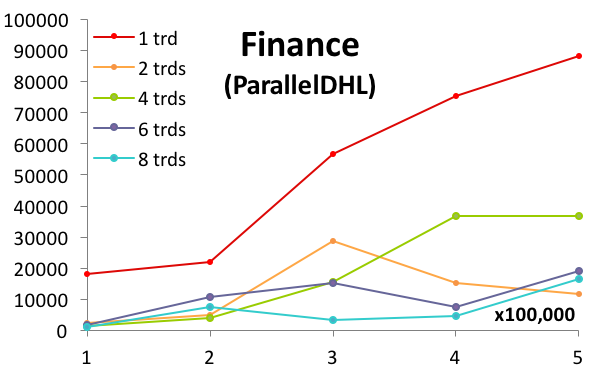
\includegraphics[width=\textwidth]{experimentalResults/1-Finance-simple}
    \subcaption{lg1\label{fig:financepdhl}} 
  \end{minipage}
  \begin{minipage}{.24\textwidth}
    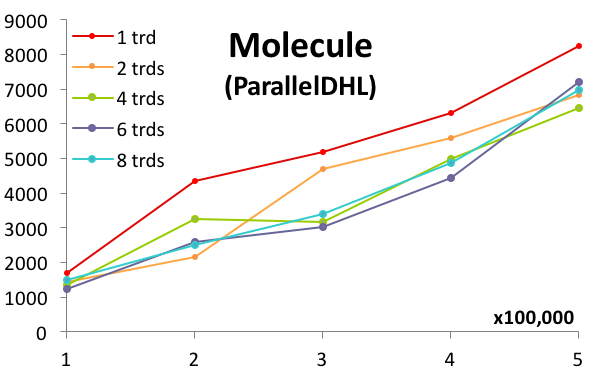
\includegraphics[width=\textwidth]{experimentalResults/2-molecule-simple}
    \subcaption{lg3\label{fig:moleculepdhl}}
  \end{minipage}
  \begin{minipage}{.24\textwidth}
    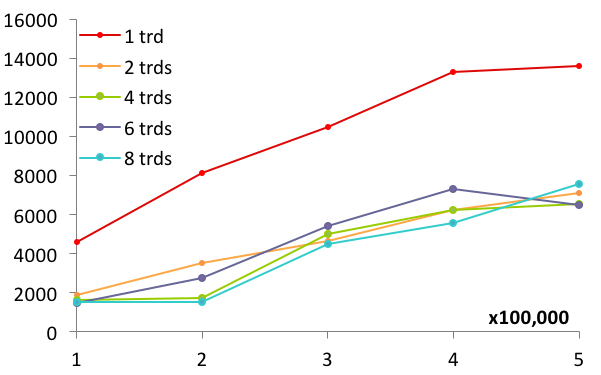
\includegraphics[width=\textwidth]{experimentalResults/3-NIF_GrossAnatomy-simple}
    \subcaption{lg5\label{fig:grossanatomypdhl}}
  \end{minipage}
  \begin{minipage}{.24\textwidth}
    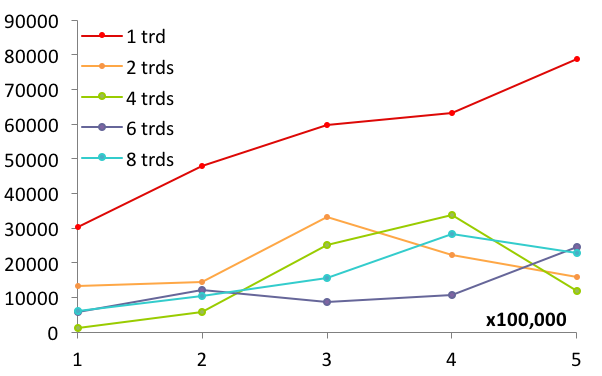
\includegraphics[width=\textwidth]{experimentalResults/4-skeleton-simple}
    \subcaption{lg7\label{fig:skeletonpdhl}}
  \end{minipage}
  \caption{Materialization time in ms for ParallelDHL for the
    ontologies that do not belonging to $\mathcal{D}_{\textit{\text{dhl}}(\circ)}$.~\label{fig:eval}}
\end{figure}

\begin{figure}[htbp]
  \centering
  \begin{minipage}{.5\textwidth}
    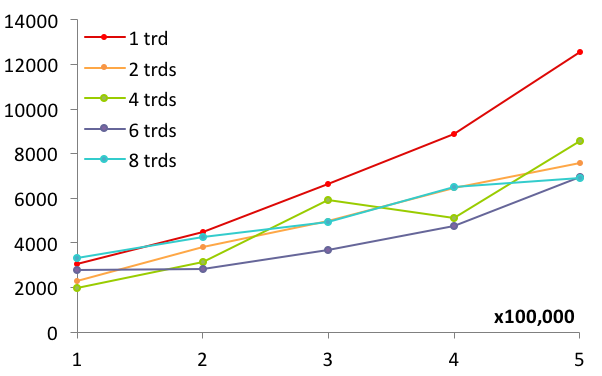
\includegraphics[width=\textwidth]{experimentalResults/1-Finance-rdfox}
    \subcaption{lg2\label{fig:financerdfox}} 
  \end{minipage}
  \begin{minipage}{.5\textwidth}
    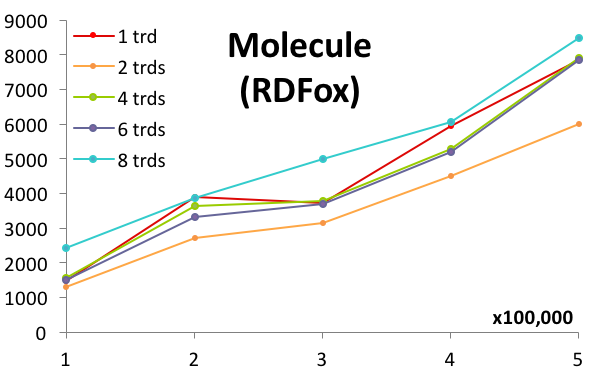
\includegraphics[width=\textwidth]{experimentalResults/2-molecule-rdfox}
    \subcaption{lg4\label{fig:moleculerdfox}}
  \end{minipage}\\
  \begin{minipage}{.5\textwidth}
    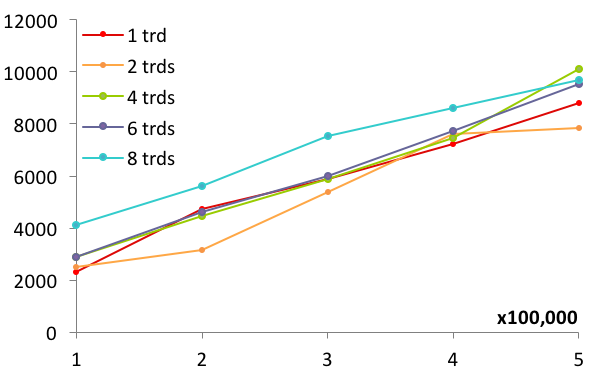
\includegraphics[width=\textwidth]{experimentalResults/3-NIF_GrossAnatomy-rdfox}
    \subcaption{lg6\label{fig:grossanatomyrdfox}}
  \end{minipage}
  \begin{minipage}{.5\textwidth}
    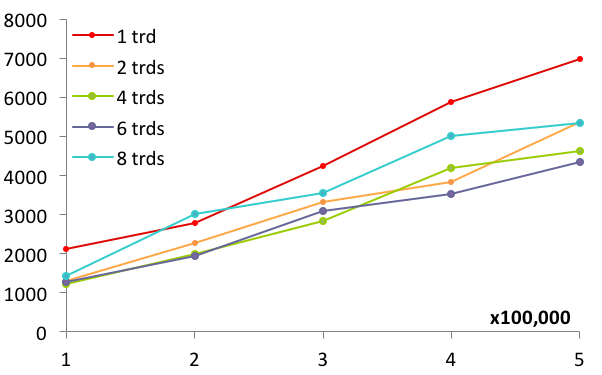
\includegraphics[width=\textwidth]{experimentalResults/4-skeleton-rdfox}
    \subcaption{lg8\label{fig:skeletonrdfox}}
  \end{minipage}
  \caption{Materialization time in ms for RDFox for the
    ontologies that do not belonging to $\mathcal{D}_{\textit{\text{dhl}}(\circ)}$.~\label{fig:eval}}
\end{figure}

%%% Local Variables:
%%% mode: latex
%%% TeX-master: "parallel-tractability-J"
%%% End:
